\newpage

\section{Convert your TGG to textual syntax}
\genHeader

Your ``old'' TGG specified with EA (visual syntax) can easily be
converted to our new textual syntax:

\begin{enumerate}

\item[$\blacktriangleright$] In Eclipse, navigate to the \texttt{model} folder
of your TGG project and right click on the \texttt{pre.tgg.xmi} file
(\texttt{<your TGG>.pre.tgg.xmi}).
Choose \texttt{Convert to MOSL} from the eMoflon context menu
(Figure~\ref{fig:convertToMOSL}).


\item[$\blacktriangleright$] In \texttt{src/org.moflon.tgg.mosl}, check the
created \texttt{.tgg} file which represents your TGG in textual syntax.
(Figure~\ref{fig:tggfile}).
\end{enumerate}

\begin{figure}[h]
\begin{center}
 	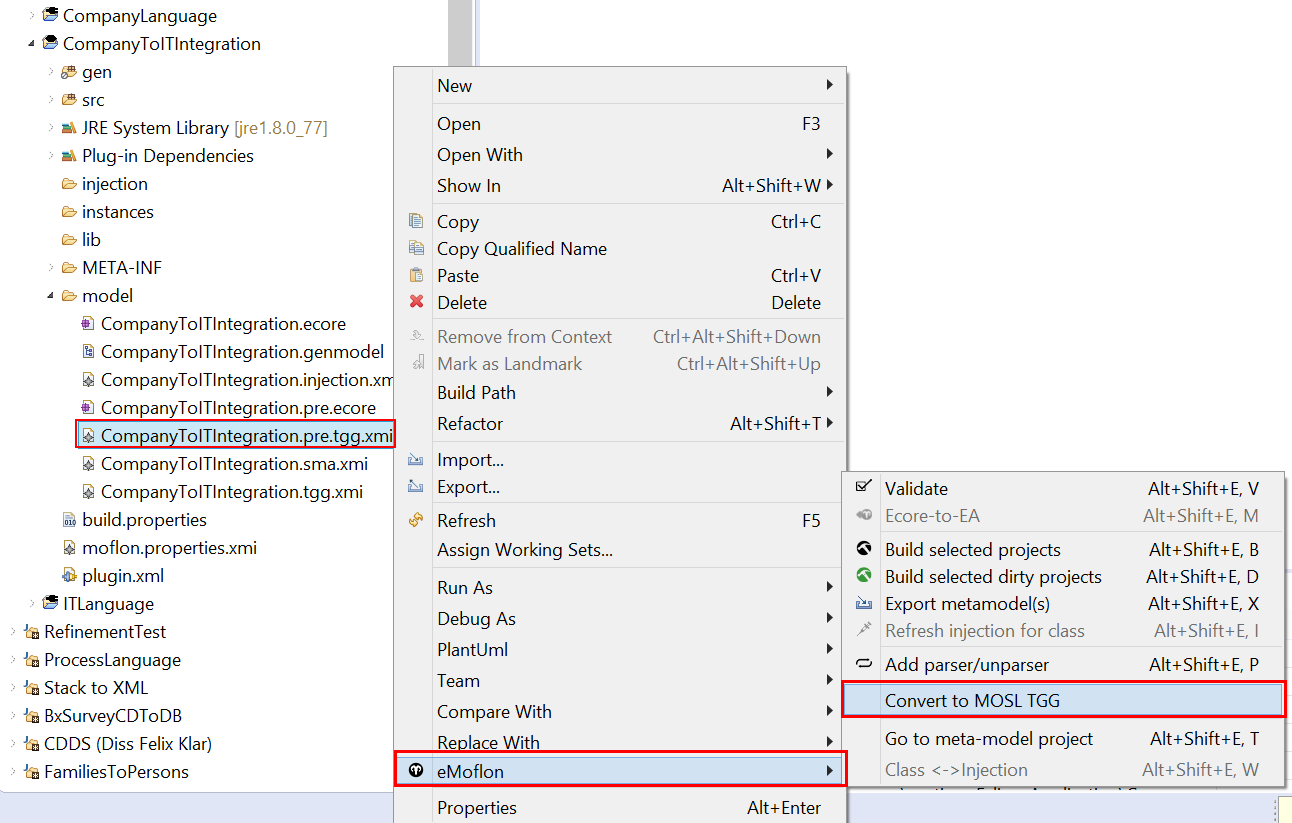
\includegraphics[width=\textwidth]{convertToMOSL}
	\caption{Convert your TGG to textual syntax}
  	\label{fig:convertToMOSL}
\end{center}

\end{figure}
\begin{figure}[h]
\begin{center}
 	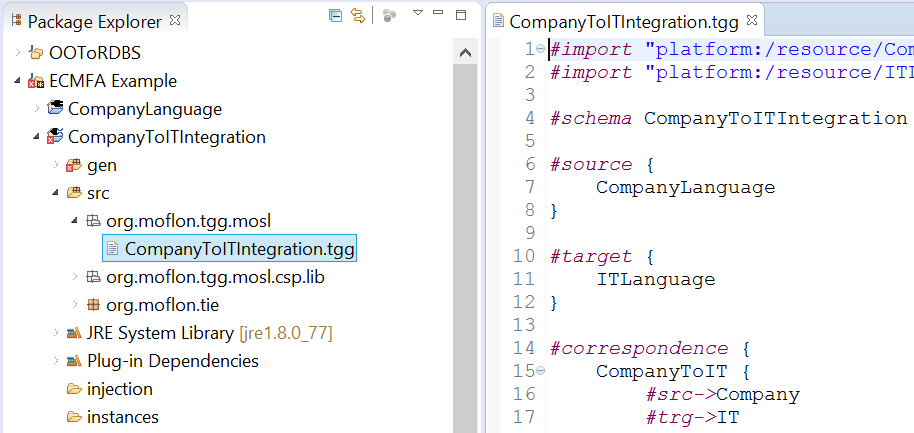
\includegraphics[width=0.7\textwidth]{tggfile}
	\caption{The created \texttt{.tgg} file representing your TGG in textual
	syntax}
  	\label{fig:tggfile}
\end{center}
\end{figure}

If you are not familiar with the textual syntax, the best thing you can do is 